\begin{frame}{Est-on d'accord?}
  \begin{columns}
    \column{0.4\textwidth}
      \begin{itemize}
        \item[E1:] Il y a combien de \underline{\uncover<2>{boîtes de pizza}}?
        \item[E2:] Il y a \underline{\uncover<2>{quatre boîtes de pizza}}.
        \item[E3:] Oui, il y en a \underline{\uncover<2>{quatre}}.
      \end{itemize}
    \column{0.6\textwidth}
      \begin{minipage}[c][0.6\textheight]{\linewidth}
        \begin{center}
          \only<-2>{
            
\includegraphics[scale=0.25]{pizza_boxes.jpg}
          }
          \only<3>{
            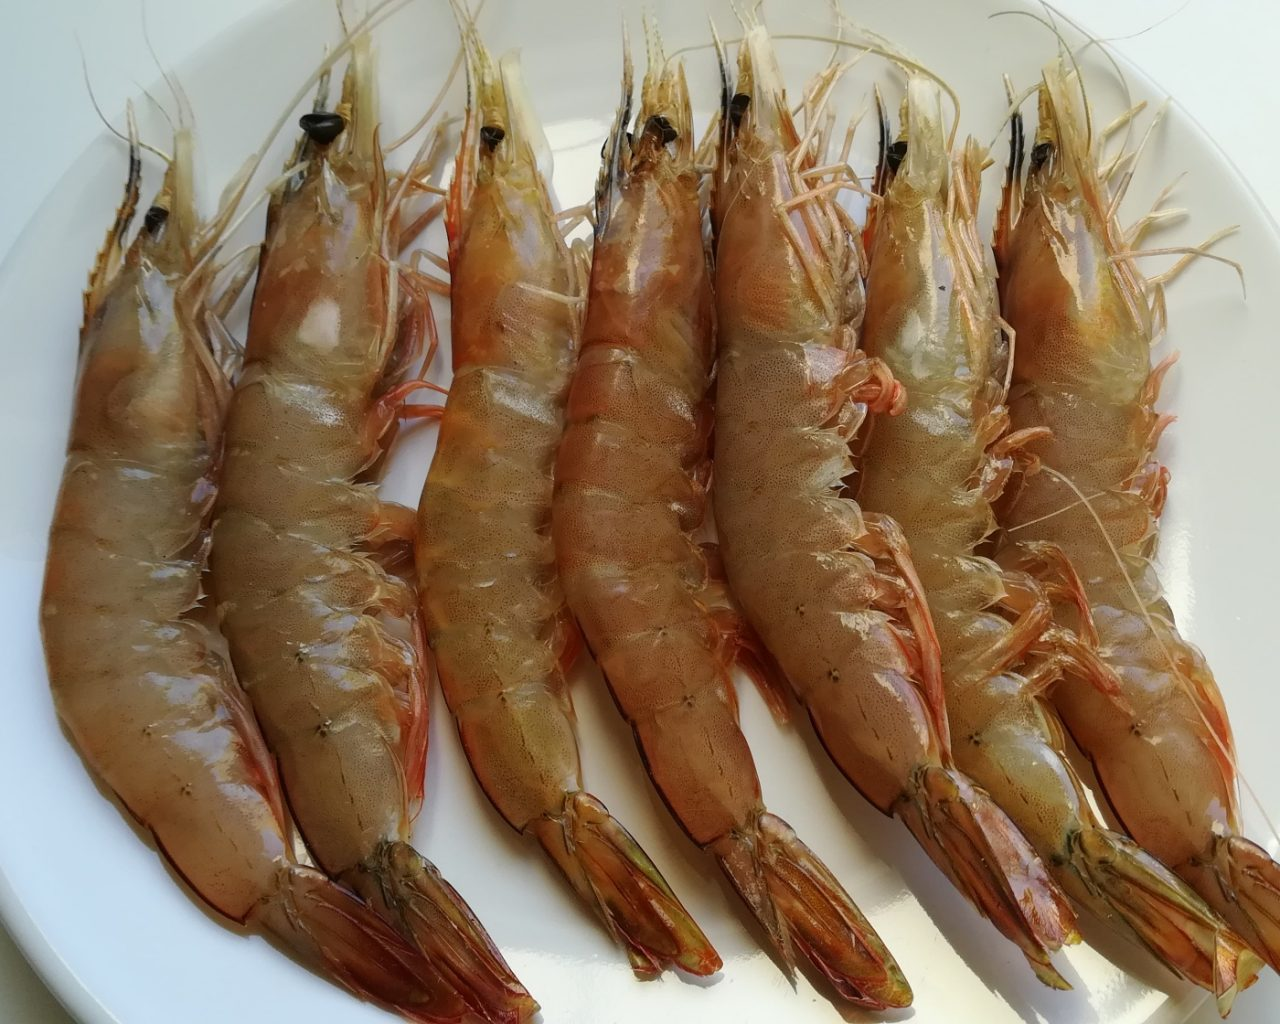
\includegraphics[scale=0.15]{crevettes.jpg}
          }
          \only<4>{
            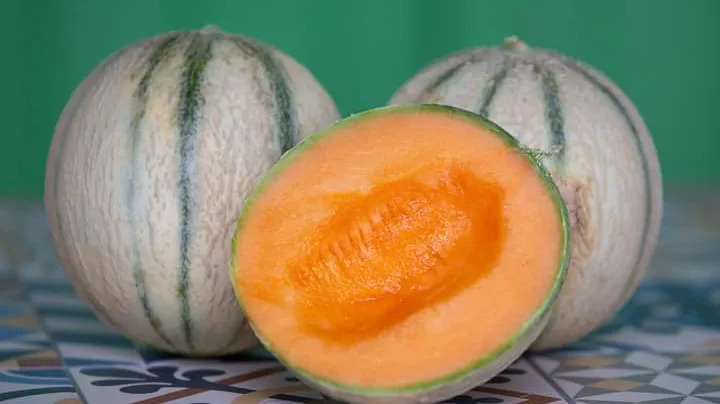
\includegraphics[scale=0.28]{melons.jpg}
          }
          \only<5>{
            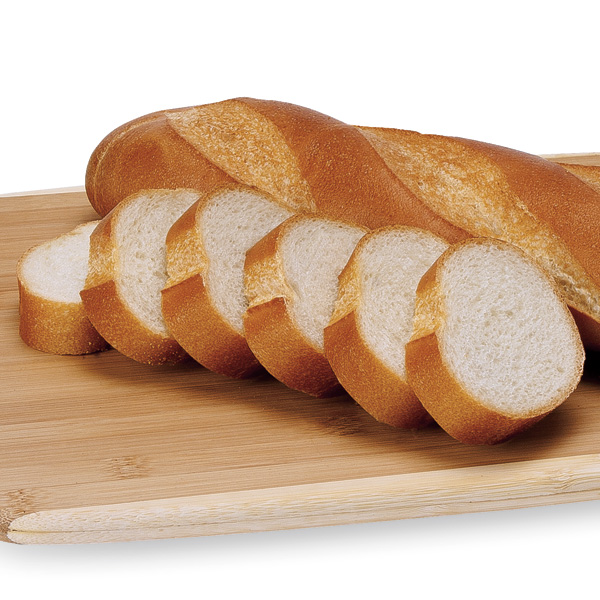
\includegraphics{tranches.jpg}
          }
          \only<6>{
            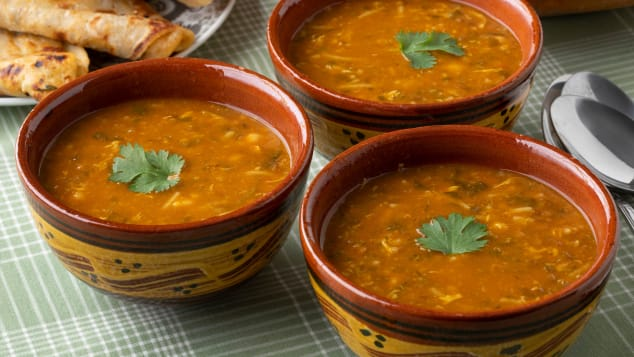
\includegraphics[scale=0.33]{bols.jpg}
          }
          \only<7>{
            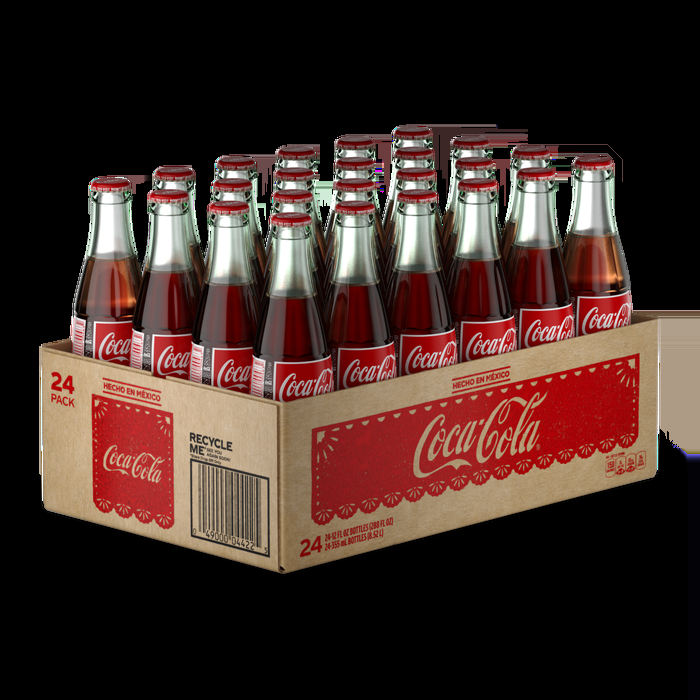
\includegraphics[scale=0.28]{bouteilles.jpg}
          }
        \end{center}
      \end{minipage}
  \end{columns}
\end{frame}